\item[6] To prevent himself from eating too many late-night snacks while preparing lecture notes, Geoff installed an electronic lock on his refrigerator door. The lock comes with an alphabetic keypad, and the door remains locked unless the last eleven letters typed form the word "CHIMICHANGA". Geoff loves chimichangas!

Design a Deterministic Finite-state Automaton (DFA) which takes in a string $s$ of alphabetic uppercase characters, and accepts $s$ if and only if it ends with CHIMICHANGA. You \textbf{must} describe the  meaning of each state in your DFA.

You can label an edge with the word ``else'' to indicate it would contain every character that does not appear on another edge leaving from the same state. For instance, if a state has outgoing edges labeled ``A'', ``B'', ``E'', ``P'' and ``else'', then ``else'' stands for ``C, D, F, G, H, I, J, K, L, M, N, O, Q, R, S, T, U, V, W, X, Y, Z''. Hint: our solution has 12 states.
\\
{\color{NavyBlue}
\\ Here is a DFA that works. We used 12 states just like the hint states. Here are the ideas:

\begin{itemize}
  \item We know that it can have any strings before the word CHIMICHAGA, so unless it starts to spell the word, there can be an initial state where the rest of the strings can be in. This is the state in the center of the diagram below.
  \item The last letters of the string has to be CHIMICHANGA, in this order, so the state after A has to be an accepting state and redirects to the initial state if there's anymore letters input. These are the states circling around the initial state in the diagram below.
  \item If the letters don't spell CHIMICHANGA exactly until the end, then it has to redirect to the initial state to restart spelling the word again, since we want that exact order. These are the lines drawing back to the state in the center in the diagram below.
  \item The word can be restarted at any point in the string, so all the states redirect to the first C state if "C" is detected as input at any point. 
  \item The second "CH" in CHIMICHANGA could also redirect back with "I" as input (for example: CHIMICHIMICHANGA is a valid input).
  \end{itemize}
  \\
\\We need 11 states to check for the exact order of the letters in the word CHIMICHANGA, and 1 initial state for all the letters before the word CHIMICHANGA to be accepted.
\\
}
\begin{center}
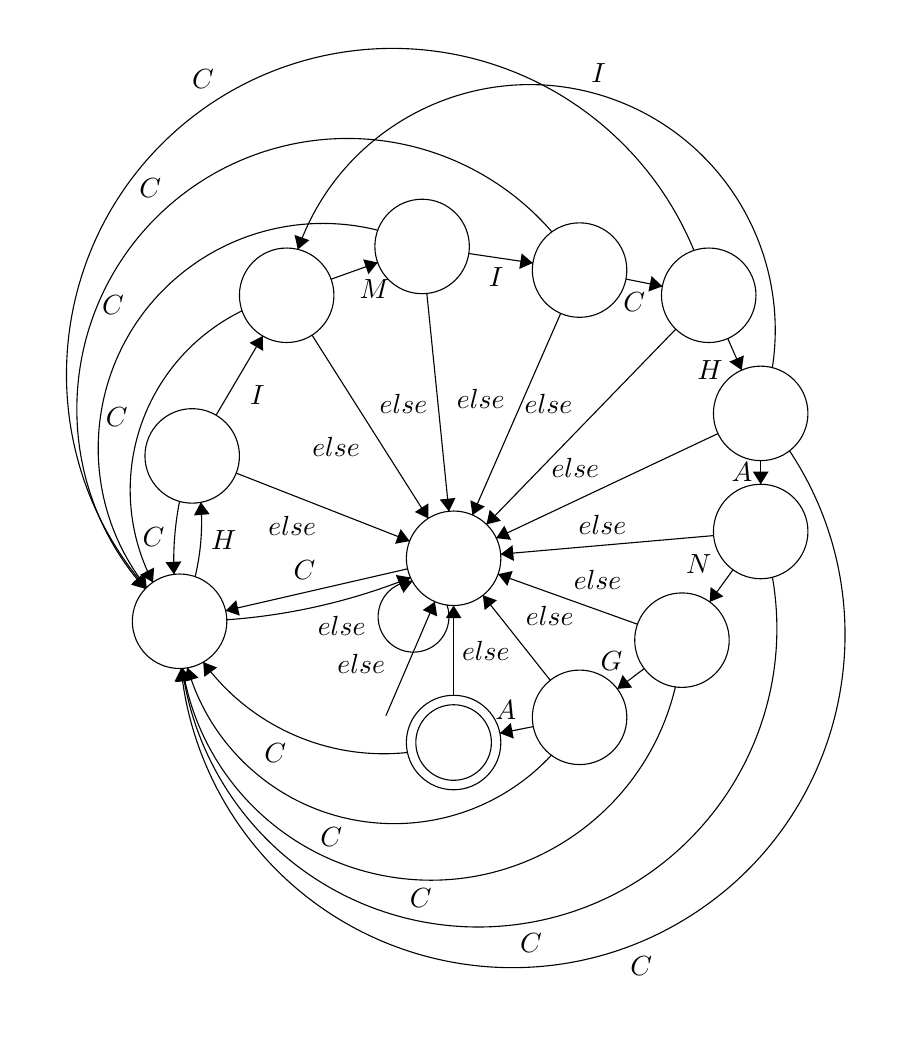
\begin{tikzpicture}[scale=0.2]
\tikzstyle{every node}+=[inner sep=0pt]
\draw [black] (32.9,-32.7) circle (3);
\draw [black] (15.5,-36.7) circle (3);
\draw [black] (16.3,-26.2) circle (3);
\draw [black] (22.3,-16) circle (3);
\draw [black] (30.9,-12.9) circle (3);
\draw [black] (40.9,-14.4) circle (3);
\draw [black] (49.1,-16) circle (3);
\draw [black] (52.4,-23.5) circle (3);
\draw [black] (52.4,-31) circle (3);
\draw [black] (47.4,-37.9) circle (3);
\draw [black] (40.9,-42.8) circle (3);
\draw [black] (32.9,-44.4) circle (3);
\draw [black] (32.9,-44.4) circle (2.4);
\draw [black] (28.6,-42.7) -- (31.71,-35.46);
\fill [black] (31.71,-35.46) -- (30.94,-35.99) -- (31.86,-36.39);
\draw [black] (32.475,-35.658) arc (19.55242:-268.44758:2.25);
\draw (27.03,-38.77) node [below] {$else$};
\fill [black] (30.29,-34.16) -- (29.37,-33.96) -- (29.71,-34.9);
\draw [black] (16.847,-29.145) arc (4.76774:-13.48169:14.949);
\fill [black] (16.85,-29.14) -- (16.41,-29.98) -- (17.41,-29.9);
\draw (17.47,-31.57) node [right] {$H$};
\draw [black] (17.82,-23.61) -- (20.78,-18.59);
\fill [black] (20.78,-18.59) -- (19.94,-19.02) -- (20.8,-19.53);
\draw (19.95,-22.35) node [right] {$I$};
\draw [black] (25.12,-14.98) -- (28.08,-13.92);
\fill [black] (28.08,-13.92) -- (27.16,-13.72) -- (27.49,-14.66);
\draw (27.88,-14.99) node [below] {$M$};
\draw [black] (33.87,-13.35) -- (37.93,-13.95);
\fill [black] (37.93,-13.95) -- (37.22,-13.34) -- (37.07,-14.33);
\draw (35.59,-14.23) node [below] {$I$};
\draw [black] (43.84,-14.97) -- (46.16,-15.43);
\fill [black] (46.16,-15.43) -- (45.47,-14.78) -- (45.27,-15.76);
\draw (44.37,-15.8) node [below] {$C$};
\draw [black] (50.31,-18.75) -- (51.19,-20.75);
\fill [black] (51.19,-20.75) -- (51.33,-19.82) -- (50.41,-20.22);
\draw (50.02,-20.73) node [left] {$H$};
\draw [black] (52.4,-26.5) -- (52.4,-28);
\fill [black] (52.4,-28) -- (52.9,-27.2) -- (51.9,-27.2);
\draw (51.9,-27.25) node [left] {$A$};
\draw [black] (50.64,-33.43) -- (49.16,-35.47);
\fill [black] (49.16,-35.47) -- (50.03,-35.12) -- (49.22,-34.53);
\draw (49.31,-33.07) node [left] {$N$};
\draw [black] (45,-39.71) -- (43.3,-40.99);
\fill [black] (43.3,-40.99) -- (44.24,-40.91) -- (43.63,-40.11);
\draw (42.92,-39.85) node [above] {$G$};
\draw [black] (37.96,-43.39) -- (35.84,-43.81);
\fill [black] (35.84,-43.81) -- (36.72,-44.15) -- (36.53,-43.16);
\draw (36.21,-42.99) node [above] {$A$};
\draw [black] (29.98,-33.37) -- (18.42,-36.03);
\fill [black] (18.42,-36.03) -- (19.32,-36.34) -- (19.09,-35.36);
\draw (23.43,-34.11) node [above] {$C$};
\draw [black] (19.09,-27.29) -- (30.11,-31.61);
\fill [black] (30.11,-31.61) -- (29.54,-30.85) -- (29.18,-31.78);
\draw (22.65,-29.99) node [below] {$else$};
\draw [black] (23.91,-18.53) -- (31.29,-30.17);
\fill [black] (31.29,-30.17) -- (31.29,-29.22) -- (30.44,-29.76);
\draw (26.98,-25.65) node [left] {$else$};
\draw [black] (31.2,-15.88) -- (32.6,-29.72);
\fill [black] (32.6,-29.72) -- (33.02,-28.87) -- (32.02,-28.97);
\draw (31.26,-22.89) node [left] {$else$};
\draw [black] (39.7,-17.15) -- (34.1,-29.95);
\fill [black] (34.1,-29.95) -- (34.88,-29.42) -- (33.96,-29.02);
\draw (36.17,-22.58) node [left] {$else$};
\draw [black] (47.01,-18.15) -- (34.99,-30.55);
\fill [black] (34.99,-30.55) -- (35.9,-30.32) -- (35.19,-29.62);
\draw (40.47,-22.88) node [left] {$else$};
\draw [black] (49.69,-24.78) -- (35.61,-31.42);
\fill [black] (35.61,-31.42) -- (36.55,-31.53) -- (36.12,-30.63);
\draw (40.63,-27.59) node [above] {$else$};
\draw [black] (49.41,-31.26) -- (35.89,-32.44);
\fill [black] (35.89,-32.44) -- (36.73,-32.87) -- (36.64,-31.87);
\draw (42.35,-31.2) node [above] {$else$};
\draw [black] (44.58,-36.89) -- (35.72,-33.71);
\fill [black] (35.72,-33.71) -- (36.31,-34.45) -- (36.65,-33.51);
\draw (42.04,-34.74) node [above] {$else$};
\draw [black] (39.04,-40.45) -- (34.76,-35.05);
\fill [black] (34.76,-35.05) -- (34.87,-35.99) -- (35.65,-35.37);
\draw (37.46,-36.33) node [right] {$else$};
\draw [black] (32.9,-41.4) -- (32.9,-35.7);
\fill [black] (32.9,-35.7) -- (32.4,-36.5) -- (33.4,-36.5);
\draw (33.4,-38.55) node [right] {$else$};
\draw [black] (23.009,-13.09) arc (160.80506:-8.78795:15.591);
\fill [black] (23.01,-13.09) -- (23.74,-12.5) -- (22.8,-12.17);
\draw (42.1,-2.53) node [above] {$I$};
\draw [black] (15.144,-33.724) arc (-177.55917:-191.15478:19.642);
\fill [black] (15.14,-33.72) -- (15.61,-32.9) -- (14.61,-32.95);
\draw (14.57,-31.34) node [left] {$C$};
\draw [black] (13.807,-34.232) arc (-152.35202:-244.01893:12.655);
\fill [black] (13.81,-34.23) -- (13.88,-33.29) -- (12.99,-33.75);
\draw (12.23,-23.72) node [left] {$C$};
\draw [black] (13.407,-34.559) arc (-141.67564:-284.13485:14.272);
\fill [black] (13.41,-34.56) -- (13.3,-33.62) -- (12.52,-34.24);
\draw (12,-16.64) node [left] {$C$};
\draw [black] (30.162,-33.924) arc (-68.14623:-85.96075:38.648);
\fill [black] (30.16,-33.92) -- (29.23,-33.76) -- (29.61,-34.69);
\draw (25.79,-36.38) node [below] {$else$};
\draw [black] (13.321,-34.644) arc (-138.33667:-319.10012:17.182);
\fill [black] (13.32,-34.64) -- (13.16,-33.71) -- (12.42,-34.38);
\draw (13.64,-9.82) node [above] {$C$};
\draw [black] (13.378,-34.584) arc (-139.07144:-337.65648:20.701);
\fill [black] (13.38,-34.58) -- (13.23,-33.65) -- (12.48,-34.31);
\draw (16.99,-2.9) node [above] {$C$};
\draw [black] (54.23,-25.874) arc (33.56541:-174.19875:21.136);
\fill [black] (15.59,-39.7) -- (15.17,-40.54) -- (16.17,-40.44);
\draw (44.81,-57.99) node [below] {$C$};
\draw [black] (53.145,-33.903) arc (9.85898:-172.29665:18.965);
\fill [black] (15.67,-39.69) -- (15.28,-40.55) -- (16.27,-40.42);
\draw (37.81,-56.5) node [below] {$C$};
\draw [black] (46.984,-40.867) arc (-13.36449:-170.94413:15.962);
\fill [black] (15.69,-39.69) -- (15.32,-40.56) -- (16.31,-40.4);
\draw (30.82,-53.67) node [below] {$C$};
\draw [black] (39.113,-45.202) arc (-42.93899:-164.06954:13.646);
\fill [black] (16,-39.65) -- (15.74,-40.56) -- (16.7,-40.28);
\draw (25.13,-49.76) node [below] {$C$};
\draw [black] (29.973,-45.032) arc (-83.88003:-143.8615:14.189);
\fill [black] (17,-39.29) -- (17.07,-40.23) -- (17.88,-39.64);
\draw (21.58,-44.41) node [below] {$C$};
\end{tikzpicture}
\end{center}
